\section{実験}
%----------------------------------------------------------------------

\subsection{データセット}

\textbf{OrganAMNIST} を使用した．
OrganAMNIST は MedMNIST v2 ベンチマーク\cite{MedMNIST}に含まれる医療画像データセットであり，
Liver Tumor Segmentation Benchmark（LiTS）の 3D 腹部 CT ボリュームを
体軸断（Axial view）でスライスした 2D 画像から構成される．
肝臓・腎臓・脾臓など腹部臓器を 11 クラスに分類するタスクを対象とし，
CT のハウンズフィールド値（HU）を腹部ウィンドウでグレースケール変換した
1 チャネル画像（28$\times$28 ピクセル）を用いる．
データ数は訓練 34,561 枚，検証 6,491 枚，テスト 17,778 枚（合計 58,830 枚）である．

図~\ref{fig:organamnist}に OrganAMNIST のサンプル画像を示す．
本実験では IID 設定として，訓練データを 10 台の端末に均等に分割した．

\begin{figure}[htb]
  \centering
  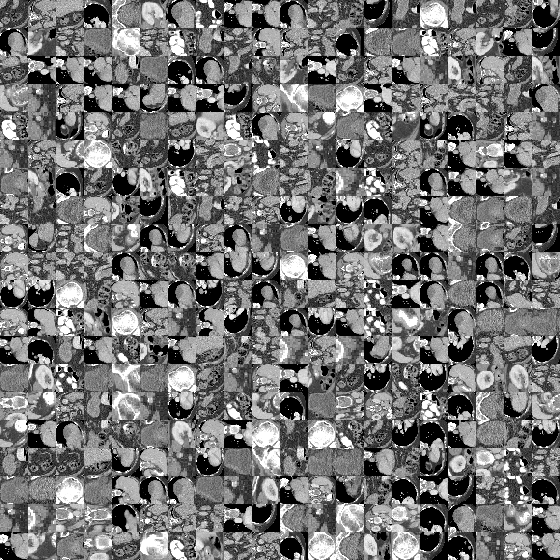
\includegraphics[width=0.85\linewidth]{figs/organamnist.png}
  \caption{OrganAMNIST のサンプル画像（28$\times$28 ピクセル，グレースケール）．
    LiTS の 3D 腹部 CT ボリュームを体軸断でスライスした画像であり，
    肝臓・腎臓・脾臓など 11 種類の腹部臓器クラスを含む．}
  \label{fig:organamnist}
\end{figure}

\subsection{端末構成}

表~\ref{tab:clients}に本実験の端末構成を示す．
10 台の端末を CNN 端末 5 台と ViT 端末 5 台に分割し，
両アーキテクチャともに縮小率を 3 段階（$r = 1.0 \times 2, 0.5 \times 2, 0.25 \times 1$）に設定することで
計算異種性とアーキテクチャ異種性の両方を再現した．

\begin{table}[htb]
  \centering
  \caption{実験における端末構成}
  \label{tab:clients}
  \begin{tabular}{llcc}
    \toprule
    端末 ID & アーキテクチャ & 縮小率 $r$ & 台数 \\
    \midrule
    C1, C2 & CNN (ResNet18) & 1.0  & 2 \\
    C3, C4 & CNN (ResNet18) & 0.5  & 2 \\
    C5     & CNN (ResNet18) & 0.25 & 1 \\
    V1, V2 & ViT-Small      & 1.0  & 2 \\
    V3, V4 & ViT-Small      & 0.5  & 2 \\
    V5     & ViT-Small      & 0.25 & 1 \\
    \bottomrule
  \end{tabular}
\end{table}

\subsection{比較手法}

以下の 2 手法と比較する．

\begin{itemize}
  \item \textbf{HeteroFL}\cite{HeteroFL}:
        CNN 端末（C1–C5）のみを対象とし，幅スケーリングによる計算異種性に対応する．
        ViT 端末は参加できない．

  \item \textbf{FedGen}\cite{FedGen}:
        FedGen は計算異種性に対応しないため，全端末が縮小率 $r = 1.0$
        の同一サイズモデルを使用する設定で評価した．
\end{itemize}

各手法はそれぞれの前提に従った設定（HeteroFL: CNN 端末 5 台・計算異種性あり，
FedGen: 全端末・幅均一，AFAD: 全端末・二重異種性あり）で評価し，
同一のデータセット・ラウンド数・ローカルエポック数を揃えた．
なお，HeteroFL との比較では参加端末数（CNN 5台 vs 全10台）に伴うデータ量の差が生じる．
これを本比較の前提として明示した上で，AFAD が HeteroFL と同等以上の精度を達成することをもって，
二重異種性への同時対応が精度低下を伴わないことの実証とする．

\subsection{実装・ハイパーパラメータ}

実装には Flower\cite{Flower}フレームワークと PyTorch を用い，
Ray による単一マシン上での分散シミュレーションで評価した．
主なハイパーパラメータを表~\ref{tab:hyperparams}に示す．

\begin{table}[htb]
  \centering
  \caption{主なハイパーパラメータ}
  \label{tab:hyperparams}
  \begin{tabular}{lc}
    \toprule
    パラメータ & 値 \\
    \midrule
    通信ラウンド数 & 40 \\
    ローカルエポック数 $E$ & 1 \\
    バッチサイズ & 32 \\
    学習率 & 0.01 \\
    オプティマイザ & SGD（momentum=0.9）\\
    KD 温度パラメータ $\tau$ & 1.0 \\
    KD 蒸留係数（$r=1.0$）& $\alpha = \beta = 0.5$ \\
    KD 蒸留係数（$r=0.5$）& $\alpha = \beta = 1.0$ \\
    KD 蒸留係数（$r=0.25$）& $\alpha = \beta = 2.0$ \\
    Bottleneck 次元 & 32 \\
    Generator 訓練エポック数 & 5 \\
    プロトタイプ正則化係数 $\gamma$ & 0.5 \\
    \bottomrule
  \end{tabular}
\end{table}

各手法について 40 ラウンドの連合学習を実施した．
評価指標として，各ラウンドにおける
グローバルモデル（$r=1.0$）のテスト精度（サーバ精度）を用いる．
主要な比較には 40 ラウンド中の最高サーバ精度を，
安定性の評価にはラウンド 11 以降の平均サーバ精度（Mean R11+）を用いる．

%----------------------------------------------------------------------
